\documentclass[a4paper,11pt]{article}
\input{/home/tof/Documents/Cozy/latex-include/preambule_doc.tex}
\input{/home/tof/Documents/Cozy/latex-include/preambule_commun.tex}
\newcommand{\showprof}{show them}  % comment this line if you don't want to see todo environment
\setlength{\fboxrule}{0.8pt}
\fancyhead[L]{\fbox{\Large{\textbf{ProgDyn 01}}}}

\fancyhead[C]{\textbf{Suite de Fibonacci}}
\newdate{madate}{10}{09}{2020}
%\fancyhead[R]{\displaydate{madate}} %\today
%\fancyhead[R]{Seconde - SNT}
%\fancyhead[R]{Première - NSI}
\fancyhead[R]{Terminale - NSI}
\fancyfoot[L]{\vspace{1mm}Christophe Viroulaud}
\AtEndDocument{\label{lastpage}}
\fancyfoot[C]{\textbf{Page \thepage/\pageref{lastpage}}}
\fancyfoot[R]{\includegraphics[width=2cm,align=t]{/home/tof/Documents/Cozy/latex-include/cc.png}}
\usepackage{tikz}

\begin{document}
\section{Problématique}
Dans un problème récréatif posé en 1202 par Leonardo Fibonacci, on décrit la croissance d'une population de lapins.\\
\guill{Quelqu’un a déposé un couple de lapins dans un certain lieu, clos de toutes parts, pour savoir combien de couples seraient issus de cette paire en une année, car il est dans leur nature de générer un autre couple en un seul mois, et qu’ils enfantent dans le second mois après leur naissance. \footnote{Davantage d'informations sur \url{https://tinyurl.com/wikifibo}  }}\\

Mathématiquement cette relation récursive s'écrit :
$$
F_n = \left\{
    \begin{array}{ll}
        F_0 = 0 & \mbox{si } n=0\\
        F_1=1 & \mbox{si } n=1\\
        F_{n} = F_{n-1}+F_{n-2} & \mbox{si } n>1\\
    \end{array}
    \right.
$$
\begin{center}
\shadowbox{\parbox{14cm}{\centering Comment obtenir un calcul efficace des termes de la suite?}}
\end{center}
\section{Mise en évidence du problème}
L'implémentation immédiate de la relation donne la fonction \emph{fibo}:
\lstinputlisting[firstline=9 ,lastline= 19]{"scripts/fibo.py"}
L'arbre des appels pour $n=8$ (figure \ref{fibo1}) montre la redondance des calculs.
\begin{center}
    \centering
    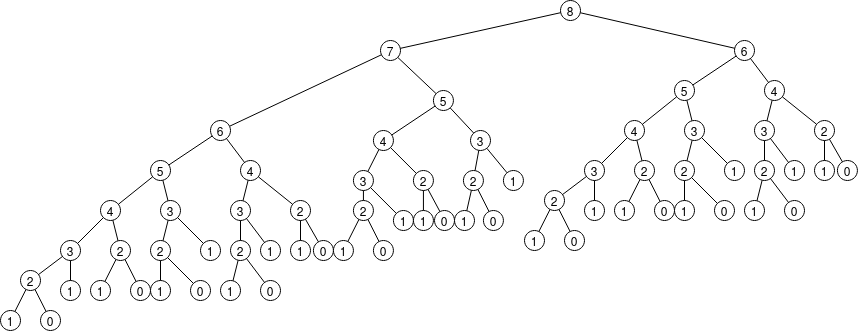
\includegraphics[width=17cm, height=7cm]{ressources/fibo1.png}
    \captionof{figure}{Appels récursifs pour $n=8$}
    \label{fibo1}
\end{center}
\begin{activite}
\begin{enumerate}
    \item Tester la fonction \emph{fibo} pour $n=8$, $n=10$.
    \item À l'aide d'une variable globale (c'est mal) \emph{compteur}, observer le nombre d'appels réalisés en fonction de \emph{n}.
\end{enumerate}
\end{activite}
\section{Programmation dynamique}
Le principe de la programmation dynamique peut être considéré comme une amélioration de l'approche \emph{diviser pour régner}. Il consiste à réutiliser des résultats déjà calculés lors du découpage en sous-problèmes.
\subsection{Top-down}
Cette approche part du problème principal (\emph{Top $\;\rightarrow\;$ Haut}) qui est découpé en petits problèmes (\emph{Down $\;\rightarrow\;$ Bas}).
\begin{center}
    \lstinputlisting[firstline=9 ,lastline= 24]{"scripts/fibo-dyn.py"}
    \captionof{code}{Approche top-down}
    \label{moncode}
\end{center}
Le tableau \emph{track} stocke les valeurs déjà calculées pour éviter d'effectuer les appels redondants.
\begin{center}
    \lstinputlisting[firstline=26 ,lastline= 28]{"scripts/fibo-dyn.py"}
    \captionof{code}{Création du tableau de mémoïsation}
    \label{moncode}
\end{center}
\begin{aretenir}[]
La \emph{mémoïsation} consiste à la \emph{mise en cache} les valeurs déjà calculées pour pouvoir être réutilisées.
\end{aretenir}
\begin{center}
    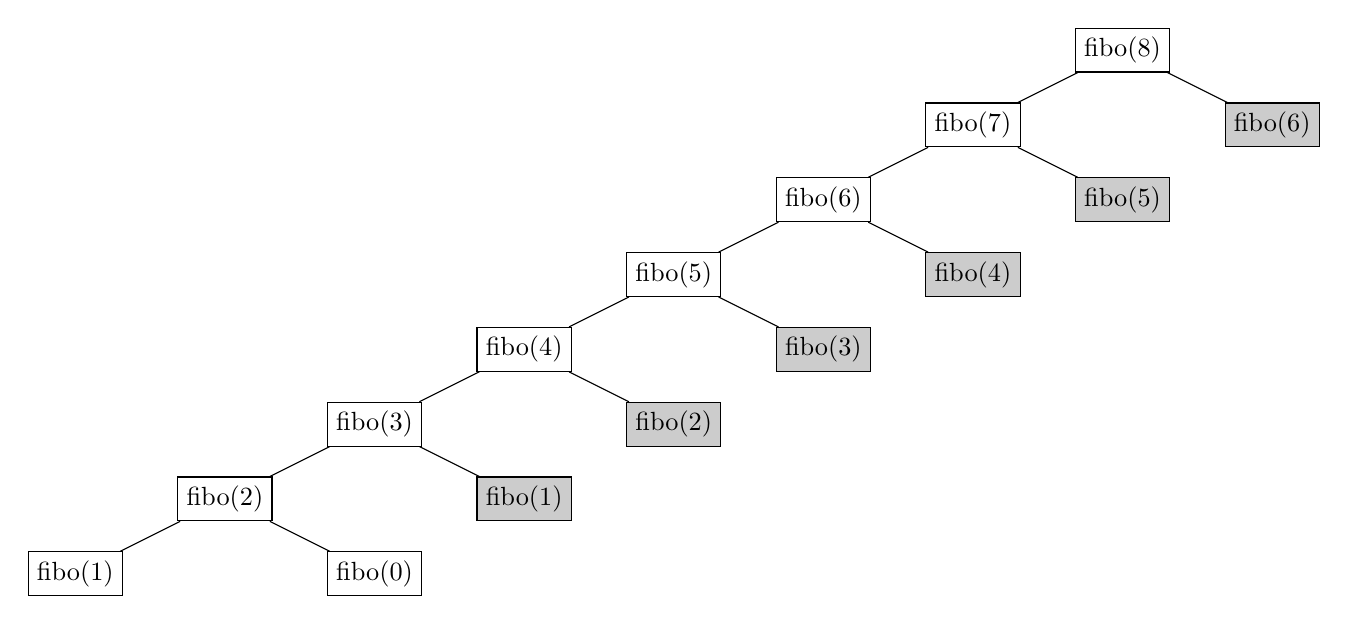
\begin{tikzpicture}[scale=0.95, transform shape]
        \node[draw] (A) at (0,0) {fibo(8)};
        \node[draw] (B) at (-2,-1) {fibo(7)};
        \node[draw,fill=gray!40] (C) at (2,-1) {fibo(6)};
        \node[draw] (D) at (-4,-2) {fibo(6)};
        \node[draw,fill=gray!40] (E) at (0,-2) {fibo(5)};
        \node[draw] (F) at (-6,-3) {fibo(5)};
        \node[draw,fill=gray!40] (H) at (-2,-3) {fibo(4)};
        \node[draw] (I) at (-8,-4) {fibo(4)};
        \node[draw,fill=gray!40] (J) at (-4,-4) {fibo(3)};
        \node[draw] (K) at (-10,-5) {fibo(3)};
        \node[draw,fill=gray!40] (M) at (-6,-5) {fibo(2)};
        \node[draw] (O) at (-12,-6) {fibo(2)};
        \node[draw,fill=gray!40] (P) at (-8,-6) {fibo(1)};
        \node[draw] (Q) at (-14,-7) {fibo(1)};
        \node[draw] (R) at (-10,-7) {fibo(0)};

        \draw (A) -- (B);
        \draw (A) -- (C);
        \draw (B) -- (D);
        \draw (B) -- (E);
        \draw (D) -- (F);
        \draw (D) -- (H);
        \draw (F) -- (I);
        \draw (F) -- (J);
        \draw (I) -- (K);
        \draw (I) -- (M);
        \draw (K) -- (O);
        \draw (K) -- (P);
        \draw (O) -- (Q);
        \draw (O) -- (R);
    \end{tikzpicture}
    \captionof{figure}{Appels récursifs pour $n=8$}
    \label{moncode}
\end{center}
\begin{activite}
Tester la fonction en approche top-down. Compter le nombre d'appels.
\end{activite}
\subsection{Bottom-up}
Cette approche \emph{itérative} résout d'abord les sous-problèmes (\emph{Bottom $\;\rightarrow\;$ Bas}) avant de remonter vers le problème principal (\emph{Up -> Haut}).
\begin{center}
    \lstinputlisting[firstline=30 ,lastline= 35]{"scripts/fibo-dyn.py"}
    \captionof{code}{Approche bottom-up}
    \label{moncode}
\end{center}
On calcule toutes les valeurs en partant de 0.

\begin{activite}
    Combien d'itérations effectue-t-on?
\end{activite}
\begin{commentprof}
top-down ou bottom-up? complexité en temps souvent identique. Complexité en espace peut varier. S'il est simple de déterminer quels résultats vont être nécessaires, l'approche bottom-up est intéressante $\;\rightarrow\;$ on ne garde que les résultats qui nous intéressent.
\end{commentprof}
\end{document}